\chapter{OpenHAB}

After analyzing the main products and services in the field of home automation and voice assistance, I must choose the solution
that can best fit this project. One of its requirements is to use as many open source and free technologies as possible, and that
the final product is easily usable by the final user and sufficiently flexible to adapt it to our needs.

OpenHAB is fully open source and completely free, and has reached a level of maturity where it is highly stable and intuitive. In its
most recent version, it provides an user interface that automatize many tasks that a standard user might not know how to do. And,
of course, it can integrate many devices from different vendors, as In have mentioned in the previous chapters, which is also one of
the most important matters for reaching our objective.

In this chapter, I will explore in depth this home automation platform and all its possibilities, in order to have a better general idea
about it when building the final system.

\section{Introduction}
As I mentioned in previous chapters, openHAB (open Home Automation Bus) is a completely free, technology agnostic and open
source platform for home automation. 

OpenHAB software is capable of integrating different domotic systems, devices and technologies into a single solution. It also
provides uniform user interfaces, and a common approach to automation rules across the entire system, regardless of the number
of manufacturers and sub-systems involved.\cite{openHABDocs}

The platform runs on many popular platforms including Linux, Windows and macOS. It is also popular to install it in systems like the
Raspberry Pi, and openHAB even provides a special distribution for this computer, called \textit{openHABian}, a simplified way of
getting up and running openHAB, but offering the complete experience.

OpenHAB defines also a community of users, contributors and maintainers, working together on the improvement of the system.
Everything related to the community is in the openHAB community forum. The community is very active and helpful, and thanks
to them I have always found a way to solve my issues.

\section{History of openHAB}
The history of openHAB begins in 2010, when Kai Kreuzer, a smart home enthusiast from Germany, developed in Java and using the
OSGi technology (Open Services Gateway Initiative) as the basis, which is a set of specifications that define a dynamic component 
system for Java. The use of this technology makes it easier to update the services independently and their implementation. It favor
the expandability of the system.

In 2013, openHAB becomes an official Eclipse project under the name of Eclipse SmartHome, but they decide to keep both projects
active and to develop them at the same time. In Eclipse SmartHome would maintain the architecture and the functionalities from the
previous openHAB, and in openHAB they would study how to integrate the different devices and technologies that it supports via 
add-ons.

The newest version, OpenHAB 2, has been the biggest change that OpenHAB has suffered since its initial launch. It includes more 
add-ons and some changes that simplify much more the process for developers, as well as implementing Apache Karaf underneath, 
which greatly extends its possibilities. In addition, the UIs have been improved, improving greatly the user experience. OpenHAB 2 is
much easier to install, and it automates many repetitive processes that might result hard for some users.

\section{Structure}
OpenHAB works thanks to add-ons, which can extend its capabilities to fit each user’s needs, from User Interfaces, to the ability to 
interact with a large and growing number of physical \textit{Things}. Add-ons may come from the OpenHAB 2 distribution, the Eclipse
SmartHome project Extensions, or from the OpenHAB 1 distribution.

\begin{figure}
	\centering
	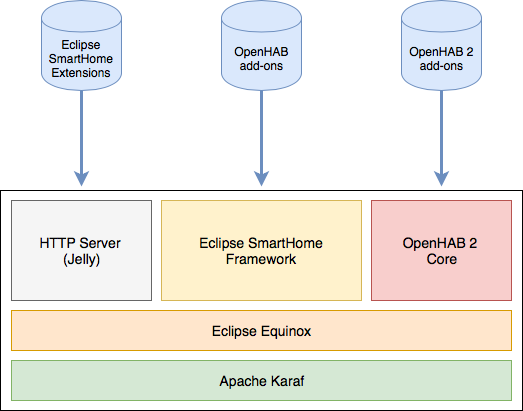
\includegraphics[width=0.9\textwidth]{images/Chapter_05/openhab-architecture.png}
	\caption{OpenHAB architecture}
	\label{fig:openhab-architecture}
\end{figure}

The figure \ref{fig:openhab-architecture} shows the overall architecture of openHAB 2. In the lowest layer, we can find Apache Karaf.
Apache Karaf is basically a modular and open source OSGi runtime environment that can host any kind of applications.\cite{apacheKaraf}
 
Next, there is Eclipse Equinox, which is also an implementation of the OSGi core framework specification. But the goal of the Equinox
project is to be a first class OSGi community and foster the vision of Eclipse as a landscape of bundles too. Equinox is responsible for
developing and delivering the OSGi framework implementation used for all of Eclipse.\cite{eclipseEquinox} 

The next and last level is divided in three parts. The first one is the Jetty HTTP server, also part of Eclipse, which provides a Web server 
and javax.servlet container, plus support for HTTP/2, WebSocket, OSGi, JMX, JNDI and JAAS, among others.\cite{eclipseJetty} Secondly,
we can find the Eclipse SmartHome Framework , the framework to build end user solutions on top like openHAB, that I mentioned 
before.\cite{eclipseSmartHomeDocs} The last part is the core of openHAB 2, which provides the full solution.

As the diagram in the figure \ref{fig:openhab-architecture} indicates, we can add to this system extensions from Eclipse SmartHome and
add-ons from the first and second version of openHAB.

